%%% Local Variables: 
%%% mode: latex
%%% TeX-master: "presentation"
%%% End: 


\begin{frame}[fragile]
  \frametitle{Motivation: Exploring High-Dim Data}
  \begin{columns}
    \column{.5\linewidth}
    \begin{itemize}
    \item<1-> Let's say you do an experiment. 
    \item<1-> You vary very few variables, and measure many different outcome variables.
    \item<1-> In our example, we change one variable, but measure four.
    \item<2-> You'd suspect there is a \alert{simple low-dimensional
      structure} hidden in these four dimensions.
    \end{itemize}
    \column{.5\linewidth}
    varied:\\
    ~\footnotesize{\verb+Y=[0,1,2,1,1,0,2,0,...]+}

    observed:
\begin{verbatim}
X =
[[ 5.1  3.5  1.4  0.2]
 [ 4.9  3.   1.4  0.2]
 [ 4.7  3.2  1.3  0.2]
 [ 4.6  3.1  1.5  0.2]
 [ 5.   3.6  1.4  0.2]
 [ 5.4  3.9  1.7  0.4]
 [ 4.6  3.4  1.4  0.3]
 [ 5.   3.4  1.5  0.2]
 [ 4.4  2.9  1.4  0.2]
 ...
 [ 4.8  3.4  1.6  0.2]
 [ 4.8  3.   1.4  0.1]
 [ 4.3  3.   1.1  0.1]]
\end{verbatim}
  \end{columns}
\end{frame}

\begin{frame}[fragile]
  \frametitle{Plotting the Data}
  \begin{columns}
    \column{.5\linewidth}
    \begin{itemize}
    \item<1-> Looking at numbers is boring.
    \item<2-> 4 dimensions can be projected make 16 pairs
    \end{itemize}
    \column{.5\linewidth}
    \begin{onlyenv}<1>
\begin{lstlisting}
X =
[[ 5.1  3.5  1.4  0.2]
 [ 4.9  3.   1.4  0.2]
 [ 4.7  3.2  1.3  0.2]
 [ 4.6  3.1  1.5  0.2]
 [ 5.   3.6  1.4  0.2]
 [ 5.4  3.9  1.7  0.4]
 [ 4.6  3.4  1.4  0.3]
 [ 5.   3.4  1.5  0.2]
 [ 4.4  2.9  1.4  0.2]
 ...
 [ 4.8  3.4  1.6  0.2]
 [ 4.8  3.   1.4  0.1]
 [ 4.3  3.   1.1  0.1]]
\end{lstlisting}
    \end{onlyenv}
    %\includegraphics<2>[width=\linewidth]{pca-pics/iris-all}
    \includegraphics<2>[width=\linewidth]{pca-pics/iris-all-nocolor}
  \end{columns}
\end{frame}

\begin{frame}[plain]
  \begin{center}
   
    %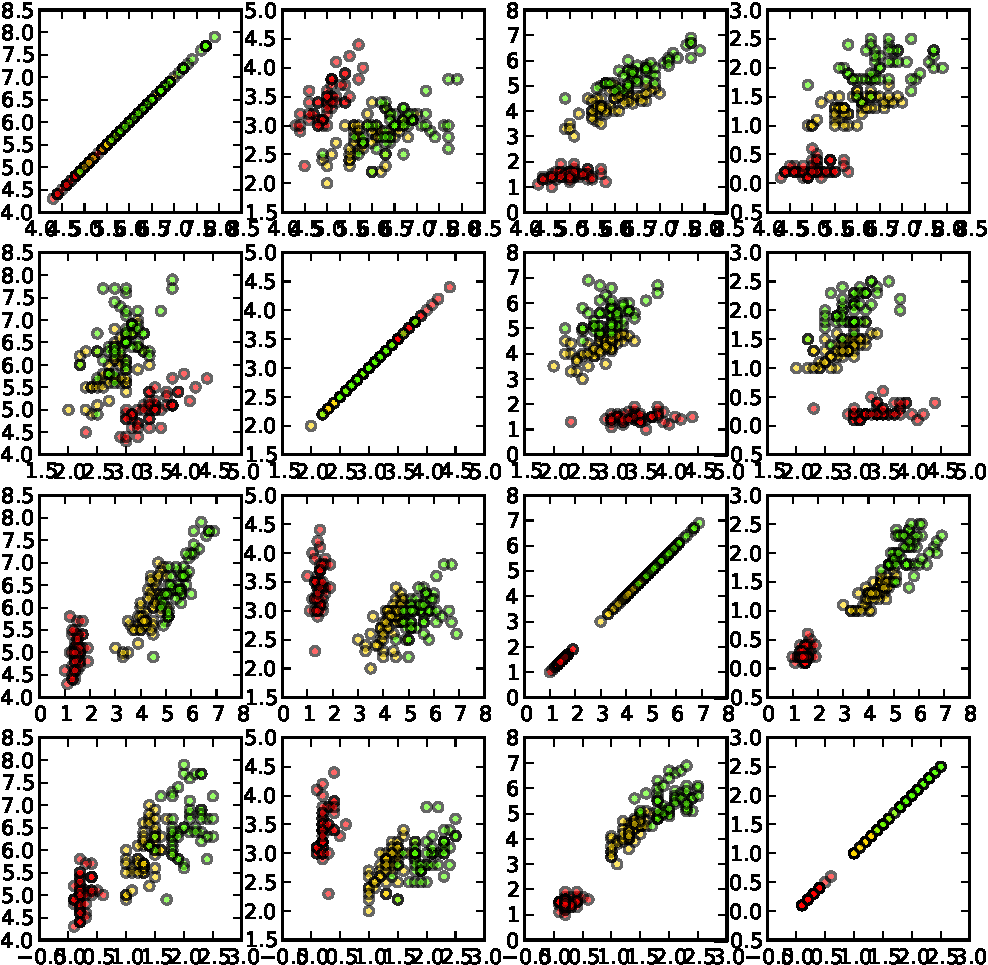
\includegraphics[height=.99\textheight]{pca-pics/iris-all}
    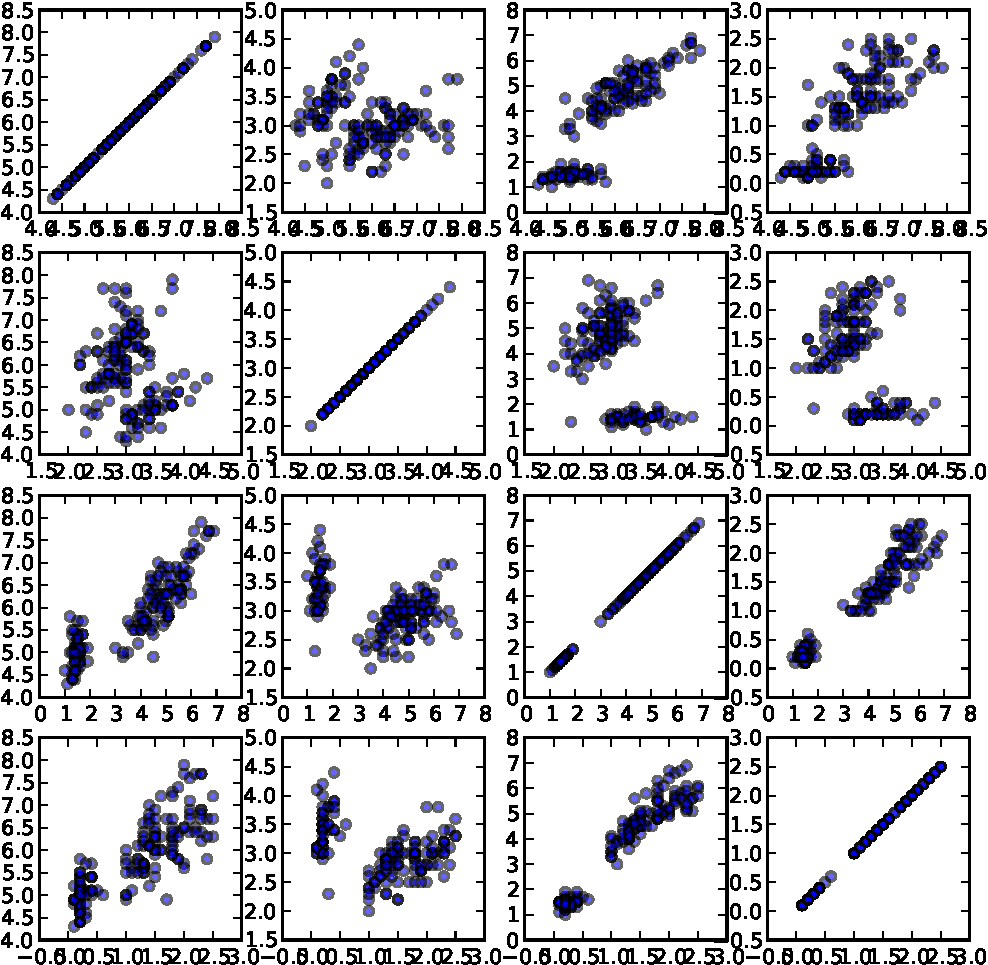
\includegraphics[height=.99\textheight]{pca-pics/iris-all-nocolor}

  \end{center}
\end{frame}

\begin{frame}
  \frametitle{Plotting the Data}
  \begin{columns}
    \column{.5\linewidth}

    \begin{enumerate}
    \item<1-> Which one of those projections is \alert{good}?
    \item<2-> Are there other, possibly \alert{better} projections?
    \item<3-> \alert{Which variables} are involved in the best
      projections?
    \end{enumerate}
    \column{.5\linewidth}
    %\includegraphics<1->[width=\linewidth]{pca-pics/iris-all}
    \includegraphics<1->[width=\linewidth]{pca-pics/iris-all-nocolor}
  \end{columns}
\end{frame}

\begin{frame}[fragile]
  \frametitle{Principal Component Analysis}
  \begin{columns}
      \begin{column}{6cm}
          \begin{itemize}[<+->]
              \item In image on right, what is the ``most important axis''?
              \item PCA models the data as a (multi-dimensional) ellipse
              \item PCA finds direction with largest variance (=diameter)
              \item First coordinate is projection onto this direction
              \item Continue with second, orthogonal axis\ldots
          \end{itemize}
      \end{column}
  
      \begin{column}{5cm}
          \includegraphics<1>[width=\linewidth]{pca-pics/pointcloud-2d}
          \includegraphics<2>[width=\linewidth]{pca-pics/pointcloud-2d-model}
          \includegraphics<3>[width=\linewidth]{pca-pics/pointcloud-2d-vecs-1a}
          \includegraphics<4>[width=\linewidth]{pca-pics/pointcloud-2d-vecs-proj1}
          \includegraphics<5>[width=\linewidth]{pca-pics/pointcloud-2d-vecs-2a}
      \end{column}
      \end{columns}
\end{frame}

\begin{frame}[fragile]
  \frametitle{Principal Component Analysis}
  \begin{columns}
      \begin{column}{6cm}
          \begin{enumerate}[<+->]
              \item Find mean
              \item Subtract mean
              \item Model as ellipse
              \item Rotate to align with axis
              \item Project data points to 1st axis\\
                  note the small error!
              \item Project data points to 2nd axis\\
                  note the larger error!
              \item \ldots
          \end{enumerate}
      \end{column}
  
      \begin{column}{5cm}
          \includegraphics<1>[width=\linewidth]{pca-pics/pointcloud-2d-step1}
          \includegraphics<2>[width=\linewidth]{pca-pics/pointcloud-2d-step2}
          \includegraphics<3>[width=\linewidth]{pca-pics/pointcloud-2d-step3}
          \includegraphics<4>[width=\linewidth]{pca-pics/pointcloud-2d-step4}
          \includegraphics<5>[width=\linewidth]{pca-pics/pointcloud-2d-step5}
          \includegraphics<6>[width=\linewidth]{pca-pics/pointcloud-2d-step6}
      \end{column}
      \end{columns}
\end{frame}

\begin{frame}[fragile]
  \frametitle{PCA Summary}
  \begin{itemize}
  \item PCA projects to axis with greatest \alert<1>{variance}
  \item Often provides good \alert<1>{first insight} into dataset
  \end{itemize}

  \begin{columns}
    \column{.5\linewidth}
    \begin{align*}
        \bar X &\leftarrow X - \mathrm{mean}(X) & \bar X&\in\mathbb R^{n{\times}N}\\
        W &\leftarrow \mathrm{PCA}(\bar X, 2) & W &\in\mathbb R^{N{\times}M}\\
        X_{\mathrm{PCA}} & \leftarrow \bar X \cdot W& 
        X_{\mathrm{PCA}}&\in\mathbb R^{n{\times}M}
    \end{align*}
    \column{.5\linewidth}
    %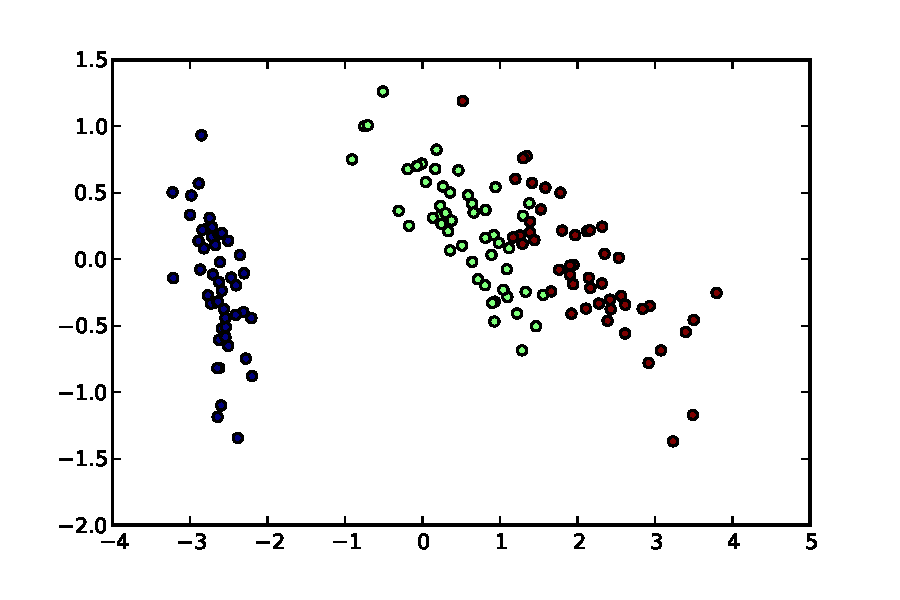
\includegraphics[width=.99\linewidth]{pca-pics/iris-2d}
    \includegraphics<1>[height=.7\linewidth]{pca-pics/iris-all-nocolor}
    \includegraphics<2->[height=.7\linewidth]{pca-pics/iris-2d-nocolor}
  \end{columns}

  \uncover<3->{%
  \begin{itemize}
  \item Identify important variables in projection matrix $W$:
  \end{itemize}

  \texttt{%
    W = [[ 0.36 -0.08 \alert<3>{0.85} 0.35] \\
    ~~~~~[\alert<4>{-0.65} \alert<4>{-0.72}  0.17  0.07]]\\
     }
  }
\end{frame}

\begin{frame}[fragile]
  \frametitle{Noise Reduction}
  \begin{columns}
      \begin{column}{.7\linewidth}
          \begin{itemize}
              \item Most of the data explained by first axes
              \item (almost) constant axes thrown away
              \item Projecting back to input-space reduces noise
          \end{itemize}
      \end{column}
      \begin{column}{.3\linewidth}
          \begin{align*}
              \!\!\!\!\!\!X_{\mathrm{clean}} &\leftarrow X_{\mathrm{PCA}}\cdot W^T + \mathrm{mean}(X)
          \end{align*}
      \end{column}
  \end{columns}
  \begin{center}
    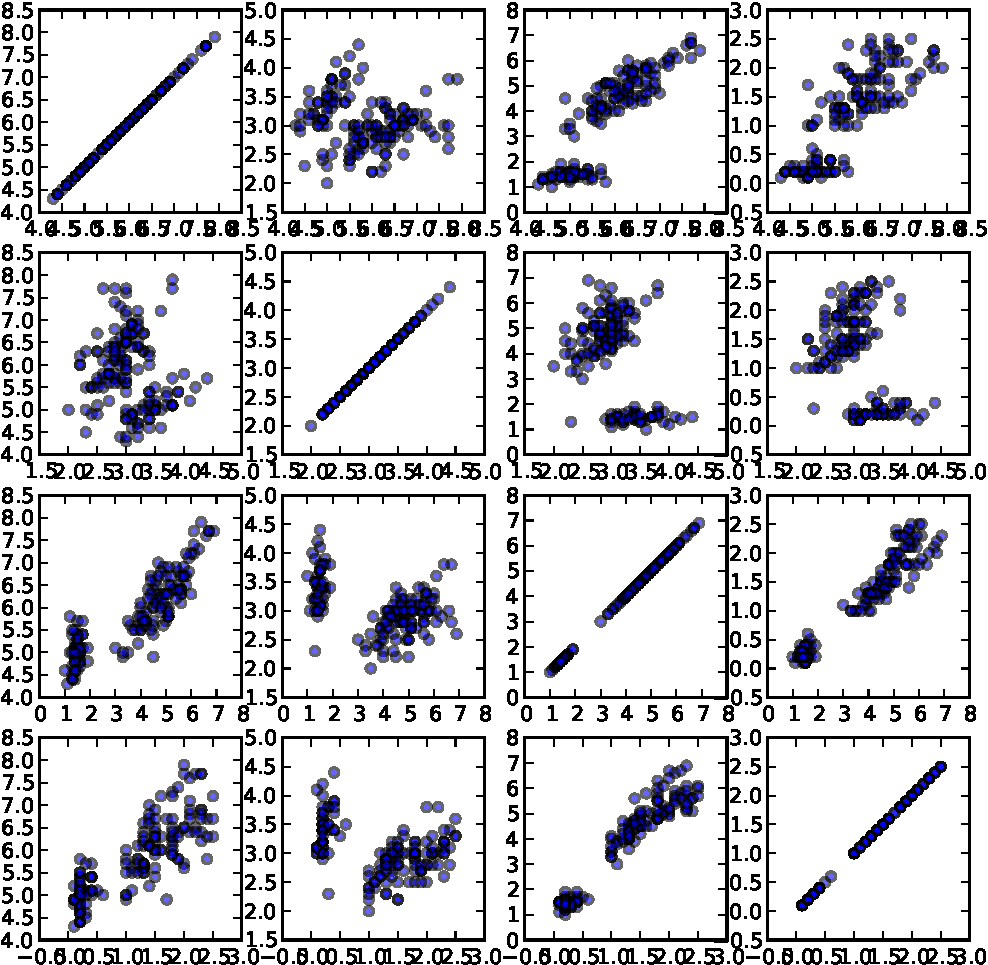
\includegraphics[width=.40\linewidth]{pca-pics/iris-all-nocolor}\hfill%
    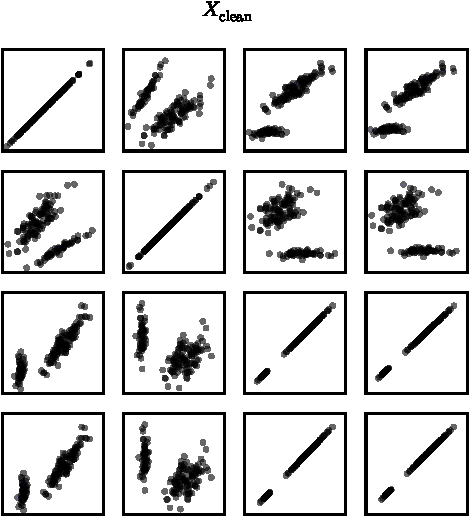
\includegraphics[width=.40\linewidth]{pca-pics/iris-bt-nocolor}
    %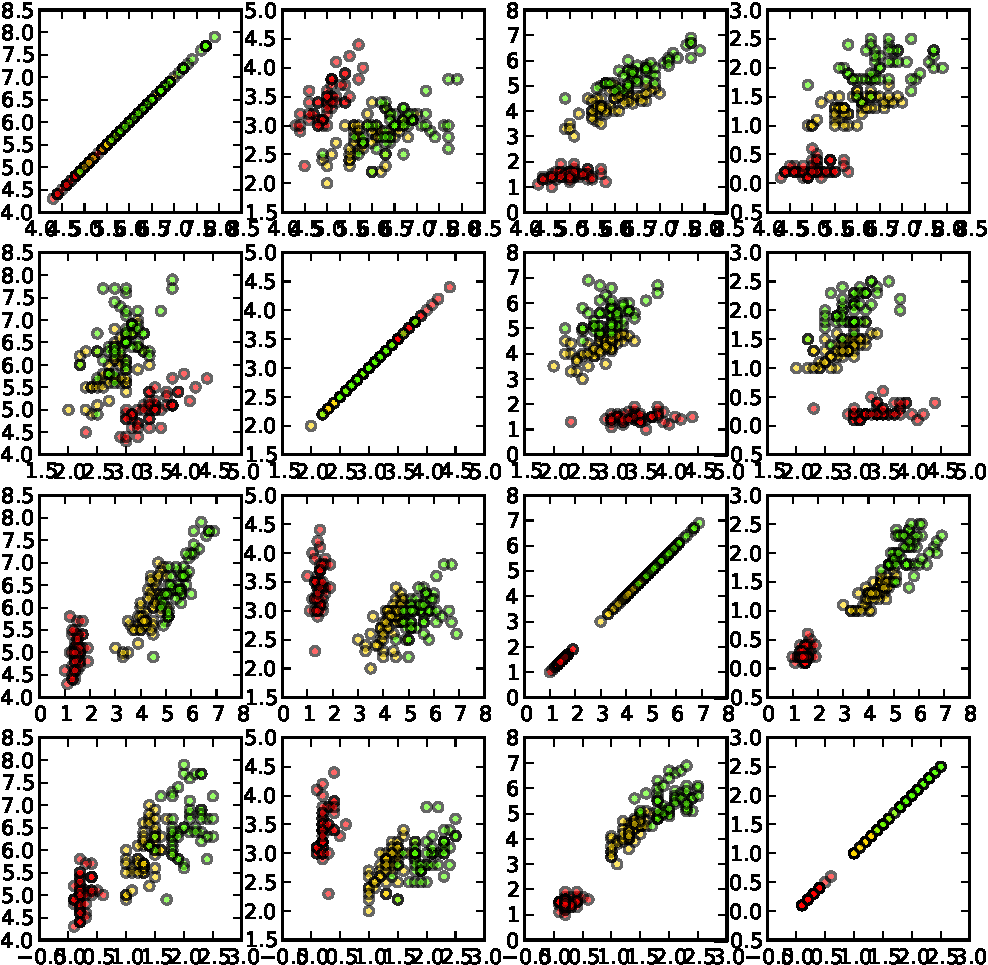
\includegraphics[width=.40\linewidth]{pca-pics/iris-all}\hfill%
    %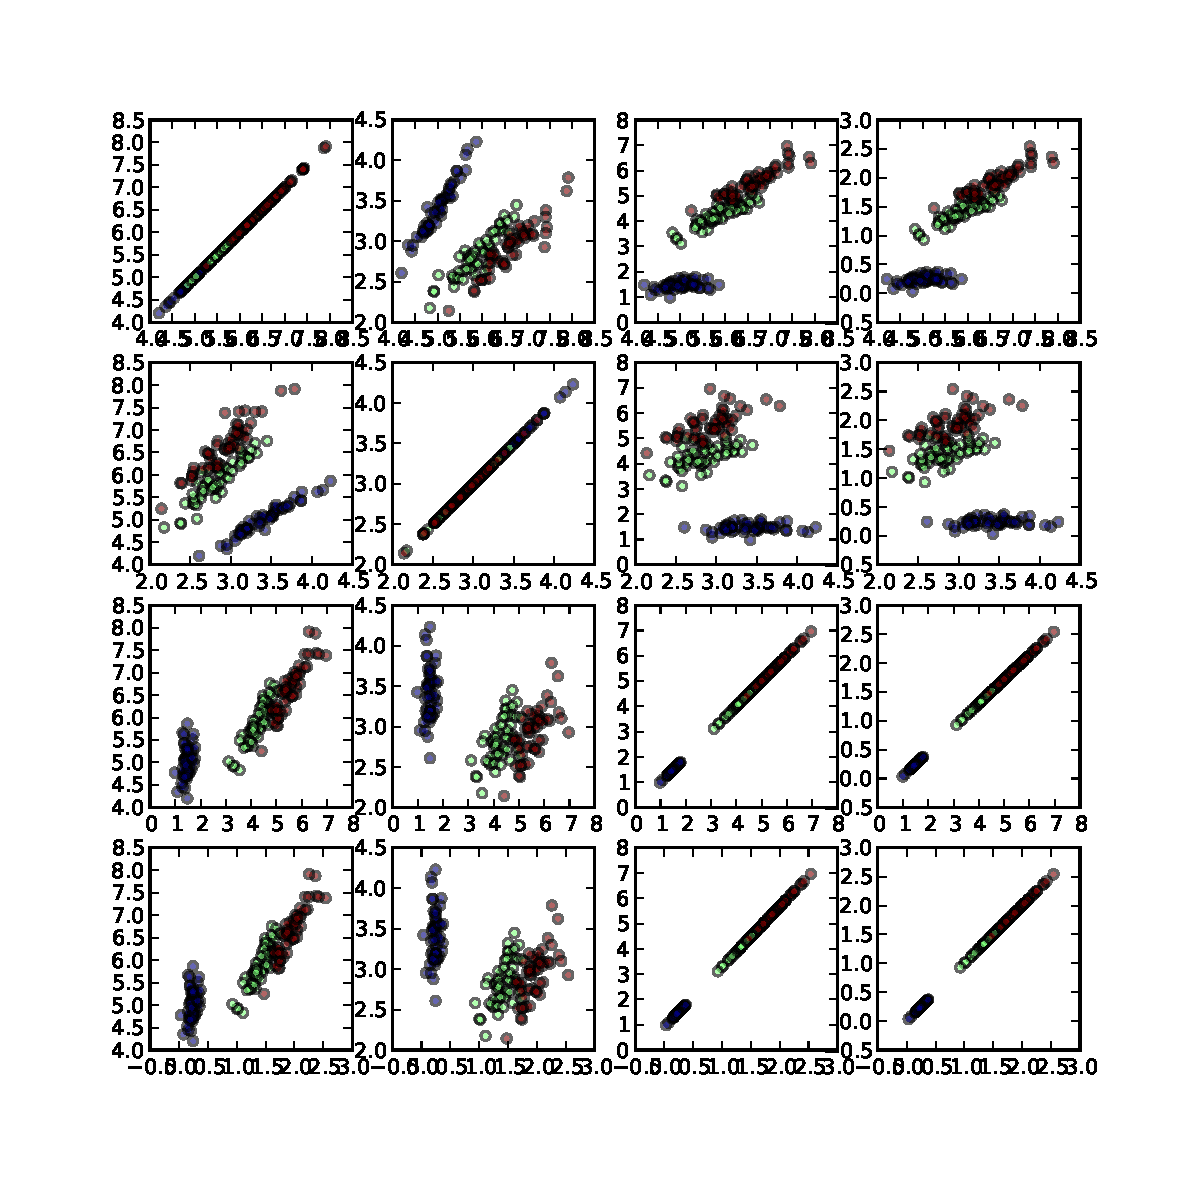
\includegraphics[width=.40\linewidth]{pca-pics/iris-bt}
  \end{center}

\end{frame}

\begin{frame}
  \frametitle{Interactive Part}
  \begin{itemize}
      \item Open Notebook titled ``1 - PCA''!
  \end{itemize}
\end{frame}


